\documentclass{datagridreport}
\usepackage{graphicx}
\usepackage{amsbsy}
\usepackage{verbatim}

\title{Automated Installation Infrastructure}
\author{Enrico Ferro \Email{enrico.ferro@pd.infn.it}}
\DocIdentifier{---}
\EDMSid{----}
\WorkPackage{WP4: Fabric Management}
\Partner{INFN}
\LeadPartner{CERN}
\DocStatus{DRAFT}
\Subtitle{}
\Dissemination{PUBLIC}

\Abstract{ Automated Installation Infrastructure provides tools to manage
large farms installation. This document describes how to setup installation
server(s), configure and install nodes}

\setlength{\parindent}{0mm}
\setlength{\parskip}{0mm}
\parindent=0mm % no paragraph indent
\parskip=0mm   % space btw paragraphs
\itemsep=0mm
\topsep=0mm

\begin{document}

\chapter{Introduction}
% ========================================================================================
Automated Installation Infrastructure manages three services:
\begin{itemize}
 \item DHCP: to distribute network configuration parameters.
 \item TFTP: to distribute Network Boot Program (NBP, the boot loader) and kernel
       images
 \item OS installer tools: to manage operating system installation.
\end{itemize}
Currently AII supports ISC-DHCP 2.0, pxelinux as NBP and RedHat 7.3.  Nodes
installation is managed via Anaconda and Kickstart files.

We suppose that the CDB server is already installed and you already setup the basic
HLD files for the nodes to install. In this document you can find:
\begin{itemize}
\item setup of an ``all-in-one'' installation server (useful for
small sites)
\item setup of a situation with more installation servers
\item customization of HLD files with all parameters needed
\item installation startup
\item tools documentation.
\end{itemize}


\chapter{Small site setup (all-in-one)} \label{allinone}
% =======================================================================================
Although AII is designed to support redundancy / load reduction by spreading
installations services in more nodes, you can concentrate all the services in just
one. This can be useful for a small site. In this situation we suppose you will
have 1 node running \emph{all} services (CDB + DHCP + TFTP + OS installer tools).
This section describes how to install all these services on the same
machine where you already installed CDB.

\section{Packages installation} \label{packages}
% ---------------------------------------------------------------------------------------
The following packages are provided by RedHat (it is likely that some of them are already
installed on your server):
\begin{itemize}
\item perl-URI
\item perl-Digest-MD5
\item perl-libwww-perl
\item perl-MIME-Base64
\item perl-HTML-Parser
\item perl-HTML-Tagset
\end{itemize}
The following packages are required by edg-aii and are provided by EDG WP4.
You can downloand them from:\\
\url{http://datagrid.in2p3.fr/distribution/datagrid/wp4/install-r3 ???}
\begin{itemize}
\item edg-perl-LC
\item edg-caf-perl
\item edg-ccm
\end{itemize}
From the same URL download and install the AII package:
\begin{itemize}
\item edg-aii
\end{itemize}

\emph{TO BE COMPLETED: nch module?}

\section{Run edg-aiisetup-all-in-one}
% ---------------------------------------------------------------------------------------
The script \texttt{\$EDG\_LOCATION/sbin/edg-aiisetup-all-in-one} is provided to automate the
installation of an all-in-one installation server. Run it to install and configure automatically
DHCP, NFS, TFTP, sudo. The script installs missing packages downloading them from a RedHat's mirror
(using the latest version on the updates section if present), creates configuration files needed
(it asks \emph{before overwriting} existing ones), starts the daemons and enables them.
The following packages will be installed:
\begin{itemize}
\item For DHCP: dhcp
\item For NBP: mtools, syslinux, xinetd, tftp-server
\item For HTTP: expat, mm, apache
\item For NFS: portmap, nfs-utils
\item For remote execution: sudo, openssh, openssh-server, openssh-clients
\end{itemize}
The directory \texttt{/osinstall/} will be used to distribute the packages and configuration
files needed for nodes installation.

\section{Complete DHCP setup}
% ---------------------------------------------------------------------------------------
\begin{enumerate}
\item Edit \texttt{/etc/dhcpd.conf} to configure your network parameters (gateway, DNS, ...).
Hosts entries will be added by the AII tool edg-dhcp but you have to write here all common parameters.
Already existing entries and manually added are preserved if they does not conflict with
the ones managed by aii-dhcp. See \texttt{man dhcpd.conf} for more details.
\item Restart dhcpd daemon \texttt{/sbin/service dhcpd restart}
\end{enumerate}

\section{Copy OS distribution}
% ---------------------------------------------------------------------------------------
\begin{enumerate}
\item Copy RedHat 7.3 distribution in \texttt{/osinstall/rh73/}
\item Copy in the TFTP accessible area the RedHat's kernel and initrd\\
\texttt{cp /osinstall/rh73/images/pxeboot/* /osinstall/nbp/rh73}
\end{enumerate}

\section{Configure AII tools} \label{confaii}
% ---------------------------------------------------------------------------------------
Edit \texttt{\$EDG\_LOCATION/etc/edg-shellfe.conf} and customize the parameter \emph{cdburl}
with the URL where the CDB is publishing the XML profiles.

\section{Configure edg-nch} \label{nch}
% ---------------------------------------------------------------------------------------
The Notification Client Handler (NCH) is run by edg-ccm-listend to receive notifications
about CDB profiles changes. You should configure it so in this way:
\begin{verbatim}
url = http://localhost/hld
[...]
actions = /opt/edg/sbin/edg-shellfe.conf --notify
\end{verbatim}

\section{Configure SSH} \label{ssh}
% ---------------------------------------------------------------------------------------
Now you can \emph{already} use the frontend edg-installfe (see \ref{installingnodes}) in your
installation server to select which nodes should be installed.

If you want you can install edg-installfe also in your personal workstation; in this
case you do not need to login into the installation server to operate. This section and
the next one describe the steps needed.

AII frontend uses Secure SHell to execute remotely others AII tools using public
key authentication. For this reason you should:
\begin{enumerate}
\item Create an user (e.g. \texttt{aii}) on the installation server and the directory
\texttt{.ssh} with the right permissions:
\begin{verbatim}
useradd aii
passwd aii
su - aii
mkdir ~/.ssh
chmod 0700 ~/.ssh
\end{verbatim}
\item If you do not have already, generate a couple of public+private keys on your
workstation. ssh will be used by edg-installfe to run remotely edg-shellfe on
the installation server(s). The following commands are for openssh using protocol version 2:
\begin{verbatim}
ssh-keygen -t dsa
scp ~/.ssh/id_dsa.pub aii@HOSTNAME:.ssh/authorized_keys2
\end{verbatim}
Of course replace HOSTNAME with the hostname of your target server.
\item You can now disable the `standard' login of the aii user on the server with:
\begin{verbatim}
usermod -L aii
\end{verbatim}
\end{enumerate}

\section{Install and configure edg-aii-installfe on your machine}\label{frontend}
% ---------------------------------------------------------------------------------------
Download and install on your machine the package edg-aii-frontend:\\
\url{http://datagrid.in2p3.fr/distribution/datagrid/wp4/install-r3 ??}\\
Edit the file \texttt{/opt/edg/etc/edg-installfe.conf} and set in the
variable \emph{servers} the hosts that have to be updated via ssh.
In you are using the "all-in-one" setup, so you can write something like
\begin{verbatim}
servers = aii@HOSTNAME
\end{verbatim}
where HOSTNAME is your installation server. If you have more servers
you should write something like:
\begin{verbatim}
servers = aii@dhcp.asdf.fi aii@nbp.asdf.fi aii@osinstaller.asdf.fi
\end{verbatim}

\chapter{``Big'' site setup}
% ======================================================================================
If you want to spread services in more nodes, you should do manually
part of the steps done by the script on each of them. A possible scenario is the following:
\begin{itemize}
\item 1 server for CDB (already installed)
\item 1 server for DHCP + NBP (TFTP server) + receive acknowledge from the install process
\item 1 servers for OS installation
\end{itemize}
\begin{figure}[htb]
  \begin{center}
    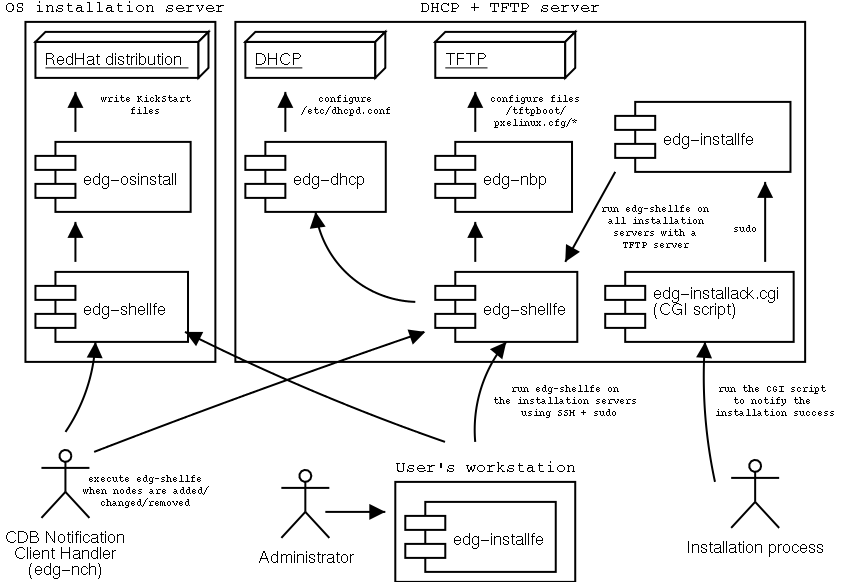
\includegraphics[width=155mm]{aii-multi.png}
  \end{center}
  \caption{Automated Installation Infrastructure: subsystem overview.}
  \label{fig:arch}
\end{figure}

This possibility is just an example, e.g. you can have more DHCP servers or
you can split the TFTP and the DHCP server. If you change the layout you should update
accordingly:
\begin{itemize}
\item The HLD files on the CDB (aii.tpl, see chapter \ref{nodesinstall})
\item The HLD configuration file (adding all the servers to be notified)
\item The configuration file of edg-installfe (which hosts are
      installation servers: edg-installfe executes edg-shellfe via
      SSH. See the man page for more details).
\end{itemize}

\section{Configure the DHCP + TFTP server}
% ---------------------------------------------------------------------------------------
\subsection{Install some RedHat packages} % ---------------------------------------------
Download and install these packages from a RedHat 7.3 mirror; check in the 'updates' section
for the latest version.
\begin{itemize}
\item For DHCP: dhcp
\item For TFTP: xinetd and tftp-server
\item For remote execution: openssh, openssh-server, sudo
\end{itemize}
A mirror:\\
\url{http://rm.mirror.garr.it/mirrors/RedHat/7.3/en/os/i386/RedHat/RPMS/}\\
\url{http://rm.mirror.garr.it/mirrors/redhat-updates/7.3/en/os/i386/}

\subsection{Install AII package and required libraries} % -------------------------------
See \ref{packages}

\subsection{Update \$PATH}\label{path} % ------------------------------------------------
If not already configured, udpate the PATH environment variable to include \$EDG\_LOCATION binary
directories by adding in \texttt{/etc/profile} the lines:
\begin{verbatim}
PATH=$PATH:/opt/edg/sbin:/opt/edg/bin
export PATH
\end{verbatim}
Of course this is in case of \$EDG\_LOCATION=/opt/edg
Log out and log in again to get the path updated.

\subsection{Configure DHCP}\label{dhcp} % ------------------------------------------------
The package edg-aii provides an example of \texttt{dhcpd.conf}: complete all network parameters
needed by your site. Enable dhcpd server and start it.
\begin{verbatim}
cp /opt/edg/share/doc/edg-aii-*/dhcpd.conf.example /etc/dhcpd.conf
vi /etc/dhcpd.conf
/sbin/chkconfig --level 2345 dhcpd on
/sbin/service dhcpd restart
\end{verbatim}
Please note that AII tools will manage  \textbf{only} the \emph{host} declarations,
so you have to prepare the file with \textbf{all other declarations} (subnet, DNS, gateway, etc...).
Of course you can add manually other host declarations that does not conflict with the
ones inserted automatically by the AII tool edg-dhcp.

\subsection{Configure SSH} % -----------------------------------------------------------
See \ref{ssh}

\subsection{Configure sudo} \label{sudo} % ----------------------------------------------
sudo is used to permit to a normal user to run a particular command with administrative
privileges. Run \texttt{visudo} and add:
\begin{verbatim}
aii    ALL=NOPASSWD:/opt/edg/sbin/edg-shellfe
apache ALL=NOPASSWD:/opt/edg/sbin/edg-installfe --boot * --nodhcp --noosinstall
\end{verbatim}

The first line is needed to execute the user commands coming from edg-installfe
frontend installed on \emph{your workstation} (see \ref{frontend}).
The second line is needed by edg-installack.cgi to run as root edg-installfe
installed on \emph{this node}. This is needed because you could have more NBP servers
that have to be notified (e.g. two NBP servers, mirrored for redundancy), so in that
situation edg-installfe is used to run in more servers edg-shellfe, and it should
be configured as described in \ref{frontend}. But in our simpler
example, edg-installfe will be just a wrapper to execute locally edg-shellfe and
you do not need to modify its configuration file \texttt{edg-installfe.conf}.

\subsection{Configure CGI script to get acknowledges} % ---------------------------------
Copy the script in cgi-bin directory and start the web server:
\begin{verbatim}
cp -f /opt/edg/sbin/edg-installack.cgi /var/www/cgi-bin/
/sbin/service httpd restart
/sbin/chkconfig --level 2345 httpd on
\end{verbatim}

\subsection{Install pxelinux and TFTP server} % -----------------------------------------
Install latest version of syslinux (unfortunately the version provided by RedHat does
not include the loader pxelinux.0) and copy the loader in a directory that will be
readable by the TFTP server:
\begin{verbatim}
rpm -Uvh ftp://ftp.kernel.org/pub/linux/utils/boot/syslinux/RPMS/syslinux-2.04-1.i386.rpm
mkdir -p /osinstall/nbp/pxelinux.cfg
cp /usr/lib/syslinux/pxelinux.0 /osinstall/nbp
\end{verbatim}
Enable TFTP server and start it:
\begin{verbatim}
cp -f /opt/edg/share/doc/edg-aii-*/tftp.example /etc/xinetd.d/tftp
/sbin/chkconfig --level 2345 xinetd on
/sbin/service xinetd restart
\end{verbatim}

\subsection{Configure AII tools} % ---------------------------------------------------
See \ref{confaii}

\subsection{Configure edg-nch} % ------------------------------------------------------
See \ref{nch}


\section{Configure OS installation server}
% --------------------------------------------------------------------------------------
\subsection{Install AII packages and libraries} % --------------------------------------
See \ref{packages}

\subsection{Update \$PATH} % -----------------------------------------------------------
See \ref{path}

\subsection{Configure SSH} % -----------------------------------------------------------
See \ref{ssh}

\subsection{Configure sudo} \label{sudo2} %--------------------------------------------
Run \texttt{visudo} to edit sudo configuration and add this line:
\begin{verbatim}
aii ALL=NOPASSWD:/opt/edg/sbin/edg-shellfe
\end{verbatim}
See \texttt{man sudoers} for more details about sudo options.

\subsection{Configure RedHat installer} \label{osinstall} % ----------------------------
Copy the contents of all RedHat 7.3 CDs in /osinstall/rh73:
\begin{verbatim}
mkdir -p /osinstall/rh73
mkdir -p /osinstall/ks
mount /mnt/cdrom
cp -r /mnt/cdrom/* /osinstall/rh73
umount /mnt/cdrom
\end{verbatim}
Copy from RedHat 7.3 the kernel and initrd images needed by PXE installations:
\begin{verbatim}
mkdir -p /osinstall/nbp/rh73
cp /osinstall/rh73/images/pxeboot/* /osinstall/nbp/rh73
\end{verbatim}
We propose to use NFS do distribute software packages for the first installation.
It is possible to use also HTTP (see \ref{nodesinstall}). Download and install
RedHat packages:
\begin{itemize}
\item portmap
\item nfs-utils
\end{itemize}
Run these commands to configure NFS service:
\begin{verbatim}
cp -f /opt/edg/share/doc/edg-aii-*/exports.example /etc/exports
/sbin/service portmap restart
/sbin/service nfs restart
/sbin/service nfslock restart
/sbin/chkconfig --level 2345 portmap on
/sbin/chkconfig --level 345 nfs on
/sbin/chkconfig --level 345 nfslock on
\end{verbatim}

\subsection{Configure AII tools}  % -----------------------------------------------------
See \ref{confaii}

\subsection{Configure edg-nch} % ------------------------------------------------------
See \ref{nch}

\section{Install and configure edg-aii-frontend on your machine}
% ---------------------------------------------------------------------------------------
See \ref{frontend}

\chapter{Nodes installation} \label{nodesinstall}
% =======================================================================================
\section{Profiles setup}
Once completed the software setup on the server, you have to prepare the
nodes profiles in the CDB. The file \texttt{/opt/edg/share/doc/edg-aii-*/aii.tpl}
provides a Pan template with configuration data needed by AII tools.
It mainly tries to ``recycle'' parameters already defined in the Global Schema [1].

All data needed by AII tools are included in the branch \texttt{/system/aii}.

\subsection{General options}
If you are using an `all-in-one' server:
\begin{itemize}
\item \texttt{aii\_server}: write here its FQDN.
\end{itemize}

If you have more installation servers:
\begin{itemize}
\item \texttt{/system/aii/server\_osinstall}: the FQDN of your OS installation server.
\item \texttt{/system/aii/osinstall\_protocol}: protocol used for the OS installation.
      Default value is "nfs". If you want, you can select "http". In this case you have to
      \begin{itemize}
      \item configure your web server so \texttt{/osinstall} is readable via web and
      the CGI script edg-ainstallack.cgi is executable (its URL is stored in
      /system/aii/osinstall/ks/ackurl).
      \item you can skip the NFS configuration described in \ref{osinstall}
      \end{itemize}
\item \texttt{/system/aii/server\_ack}: FQDN of the server that is receiving
      with the CGI script edg-installack.cgi the acknowledges of the end of install.
\item \texttt{/system/aii/ip\_server\_tftp}: IP address (\emph{not} the FQDN) of the
      TFTP server. Needed \emph{only} if your TFTP server is different from the DHCP server.
\end{itemize}

\subsection{OS install branch (/system/aii/osinstall/)}
\begin{itemize}
\item osinstall/kstemplate: kickstart template to be used (it should be present in the OS
      installation server in the directory \texttt{\$EDG\_LOCATION/lib/aii/osinstall}).
\item osinstall/ks/*: Kickstart options used to fill the
      template file (keyboard layout, language, ...).
\end{itemize}

\subsection{NBP branch (/system/aii/nbp/)}
\begin{itemize}
\item nbp/template: template of pxelinux configuration file to use (it should be
      present in the NBP server \texttt{\ EDG\_LOCATION/lib/aii/nbp}).
\item nbp/options/*: pxelinux options used to fill the template file (kernel, initial ram disk
      image, ...).
\end{itemize}

\subsection{DHCP branch (/system/aii/dhcp/)}
\begin{itemize}
\item dhcp/mac: MAC address of the network boot card
\item dhcp/ip: IP address associated to the network boot card
\item dhcp/tftpserver: TFTP server IP address (default: just
      the value already declared in /system/aii/ip\_server\_tftp
\item dhcp/addoptions: additional DHCP options (optional). Warning: they will be added
      in the host declaration of dhcpd.conf file, so do not forget ';' at the end of
      your parameter(s).
\end{itemize}


\chapter{Using AII tools} \label{installingnodes}
% =======================================================================================
\section{Select nodes with edg-installfe}
edg-installfe is the frontend to select via command line the nodes to install.
Once installed and configured the package edg-aii-installfe on your
workstation (see \ref{frontend}), if you already setup the nodes grid001 and grid002
with CDB, to install both:
\begin{verbatim}
edg-installfe --install grid001
edg-installfe --install grid002
\end{verbatim}
or you can use Perl regular expressions like:
\begin{verbatim}
edg-installfe --install 'grid0.+'
\end{verbatim}
You can specify the complete name:
\begin{verbatim}
edg-installfe --install grid001.supergrid.org
\end{verbatim}
To deactivate the installation of grid001:
\begin{verbatim}
edg-installfe --boot grid001
\end{verbatim}
To see the status of grid001 (if it is ready to be installed or not):
\begin{verbatim}
edg-installfe --status grid001
\end{verbatim}
To see the status of all nodes \emph{configured in the CDB} you can use the regexp:
\begin{verbatim}
edg-installfe --status .+
\end{verbatim}
Normally addition and removal of nodes are managed via the notification coming from
the  DB. Anyway you can do both operation manually; to force the addition of grid001
\begin{verbatim}
edg-installfe --configure grid001
\end{verbatim}
while to remove all grid* nodes:
\begin{verbatim}
edg-installfe --remove 'grid.*'
\end{verbatim}

For more details see the man page of edg-installfe.

\section{Using edg-shellfe in the installation servers} % -----------------------------
edg-installfe is just a wrapper to remotely execute on different installation servers
edg-shellfe, so in the installation servers you can execute edg-shellfe with the
command line parameters described for edg-installfe.

For more details see the man page of edg-shellfe.

\chapter{Software man pages}
% =======================================================================================
\label{edg-dhcp}
\section{edg-dhcp\label{edg-dhcp}\index{edg-dhcp}}


Add/remove host entries to an ISC DHCP server.

\subsection*{SYNOPSIS\label{edg-dhcp_SYNOPSIS}\index{edg-dhcp!SYNOPSIS}}
\begin{verbatim}
 edg-dhcp [options] <--configure <hostname> <mac> |
                     --configurelist <filename>   |
                     --remove <hostname>          |
                     --removelist <filename>      |
                     --removeall >
\end{verbatim}
\subsection*{DESCRIPTION\label{edg-dhcp_DESCRIPTION}\index{edg-dhcp!DESCRIPTION}}


edg-dhcp is a command line tool to add/remove nodes specific entries to
a ISC DHCP server. Already existing entries are preserved.
The administrator has to prepare the DHCP server configuration file with
all common network definitions and subnets declarations. The tool
add/remove/update entries to the corresponding subnet and restart the
DHCP server. A backup copy of the configuration file is created
before updating it and restarting the DHCP server.



Command line options override default values in \$EDG\_LOCATION/etc/edg-dhcp.conf.

\subsection*{COMMANDS\label{edg-dhcp_COMMANDS}\index{edg-dhcp!COMMANDS}}
\begin{description}

\item[--configure $<$hostname$>$ $<$mac$>$] \mbox{}

Configure $<$hostname$>$ in the DHCP server with the physical $<$mac$>$ address
(syntax: XX:XX:XX:XX:XX:XX). If the node is present its
configuration is removed and  replaced by the new one.


\item[--tftpserver $<$hostname$>$] \mbox{}

TFTP server (optional). Can be specified only with --configure.


\item[--addoptions $<$text$>$] \mbox{}

Additional DHCP options for the node that will be specified
inside the entry host. Can be specified only with --configure;
they should be specified between quotes, e.g.:
 edg-dhcp --configure node002 --addoptions 'filename loader.bin;'


\item[--configurelist $<$filename$>$] \mbox{}

Configure hosts listed on $<$filename$>$. Hosts have to be listed one per line
with the syntax $<$hostname$>$ $<$mac$>$ [tftpserver] [addoptions], where $<$hostname$>$
and $<$mac$>$ are mandatory. Lines with \# are comment. If a different TFTP server
should not be specified but there are additional options, use a ';'.
Additional options are written exactly as they have to written in DHCP
configuration file. An example:

\begin{verbatim}
 # You can use both : and - in the MAC address
 node1         00:80:45:6F:19:1A
 node2.qwer.fi 00-80-45:6F-19-1B  bootserver
 node3.qwer.fi 00:80:45:6F:19:1C  bootserver.qwer.fi filename "down.bin";
 node3.qwer.fi 00-80-45-6F-19-1D  ;                  filename "down.bin";
\end{verbatim}

\item[--remove $<$hostname$>$] \mbox{}

Remove $<$hostname$>$ from the DHCP server configuration.


\item[--removelist $<$filename$>$] \mbox{}

Remove hosts listed on $<$filename$>$ from the DHCP server. Hosts have to
be listed one per line. Lines with \# are comment.


\item[--removeall] \mbox{}

Remove configurations for *ALL* hosts configured. Useful only in case
of problems/test.

\end{description}
\subsection*{OPTIONS\label{edg-dhcp_OPTIONS}\index{edg-dhcp!OPTIONS}}
\begin{description}

\item[--cfgfile $<$path$>$] \mbox{}

Use the as configuration file $<$path$>$ instead of default
\$EDG\_LOCATION/etc/edg-dhcp.conf


\item[--dhcpconf $<$path$>$] \mbox{}

Configuration file for DHCP server (default: /etc/dhcpd.conf)


\item[--restartcmd $<$command$>$] \mbox{}

Command to be used to restart the server (default: /sbin/service
dhcpd restart). Should be provided between quotes, e.g.
 edg-dhcp --configurelist list --restartcmd '/sbin/mydhcpd --restart'.


\item[--norestart] \mbox{}

Update the configuration file but do not restart the server.

\end{description}
\subsection*{CONFIGURATION FILE\label{edg-dhcp_CONFIGURATION_FILE}\index{edg-dhcp!CONFIGURATION FILE}}


Default values of command lines options can be specified in the file
\$EDG\_LOCATION/etc/edg-dhcp.conf using syntax:

\begin{verbatim}
 <option> = <value>
\end{verbatim}


e.g.:

\begin{verbatim}
 dhcpconf = /etc/my_dhcpd.conf
\end{verbatim}
\subsection*{AUTHORS\label{edg-dhcp_AUTHORS}\index{edg-dhcp!AUTHORS}}


Enrico Ferro $<$enrico.ferro@pd.infn.it$>$


\label{edg-nbp}
\section{edg-nbp\label{edg-nbp}\index{edg-nbp}}


Create/remove entries for pxelinux

\subsection*{SYNOPSIS\label{edg-nbp_SYNOPSIS}\index{edg-nbp!SYNOPSIS}}
\begin{verbatim}
 edg-nbp [options] <--boot <hostname>          |
                    --bootlist <filename>      |
                    --configure <hostname> <template> [n1=v1] ... |
                    --configurelist <filename> |
                    --install <hostname>       |
                    --installlist <filename>   |
                    --remove <hostname>        |
                    --removelist <filename>    |
                    --removeall                |
                    --status <hostname>        |
                    --statuslist <filename> >
\end{verbatim}
\subsection*{DESCRIPTION\label{edg-nbp_DESCRIPTION}\index{edg-nbp!DESCRIPTION}}


edg-nbp manage configuration the Network Boot Program (NBP) pxelinux.
It creates the required configuration/symlink for an host to prepare it for
the installation or for normal; it can also remove previously added hosts.



It is normally executed by edg-shellfe but it can be run as stand-alone. Input data
can be specified via command line (for just 1 host) or via text file (for more hosts).



Command line line options override default values in \$EDG\_LOCATION/etc/edg-nbp.conf.

\subsection*{COMMANDS\label{edg-nbp_COMMANDS}\index{edg-nbp!COMMANDS}}
\begin{description}

\item[--boot $<$hostname$>$] \mbox{}

Enable for $<$hostname$>$ the boot from local disk (i.e do not reinstall
the OS).


\item[--bootlist $<$filename$>$] \mbox{}

Enable for hosts listed on $<$filename$>$ normal boot from local disk.


\item[--configure $<$hostname$>$ $<$template$>$] \textbf{[n1=v1] [n2=v2] ...}

Configure $<$hostname$>$ for NBP using $<$template$>$ as basic
configuration files. If $<$template$>$ is just a filename it will be
read from the directory specied via --nbpdir (see below,
default value: \$EDG\_LOCATION/lib/aii/nbp). The parameters to write
are expressed as couples name=value, where name is an id that
has to be present in the template (see the example at the end).



If the node is already present its configuration is simply
replaced by the new one.


\item[--configurelist $<$filename$>$] \mbox{}

Configure hosts listed on $<$filename$>$. Hosts have to be listed one per line
with the simple syntax $<$hostname$>$ $<$template$>$ [n1="v1"] [n2="v2"], where $<$hostname$>$
and $<$template$>$ are mandatory. Lines with \# are comment.
Values must be expressed between double (") quotes.
An example:

\begin{verbatim}
 # This is an unuseful comment
 node2.qwer.fi rh73-template  label="Redhat 7.3" kernel="vmlinuz-2.4.18"
 node2.qwer.fi rh90-template  label="Redhat 9.0" kernel="vmlinuz-2.4.20"
\end{verbatim}

\item[--install $<$hostname$>$] \mbox{}

Enable OS installation via network for $<$hostname$>$.


\item[--installlist $<$filename$>$] \mbox{}

Enable OS installation via network for hosts listed on $<$filename$>$.
Hosts have to be listed one per line. Lines starting with \# are comment.


\item[--remove $<$hostname$>$] \mbox{}

Remove configuration file for $<$hostname$>$.


\item[--removelist $<$filename$>$] \mbox{}

Remove configurations for hosts listed on $<$filename$>$. Hosts have to
be listed one per line. Lines starting with \# are comment.


\item[--removeall] \mbox{}

Remove configurations for *ALL* hosts configured. Useful only in case
of problems/test.


\item[--status $<$hostname$>$] \mbox{}

Report the boot status (boot from local disk/install) for $<$hostname$>$.


\item[--statuslist $<$filename$>$] \mbox{}

Report the boot status (boot from local disk/install) for hosts listed
on $<$filename$>$. Hosts have to be listed one per line. Lines starting
with \# are comment.

\end{description}
\subsection*{OPTIONS\label{edg-nbp_OPTIONS}\index{edg-nbp!OPTIONS}}
\begin{description}

\item[--bootconfig $<$filename$>$] \mbox{}

Generic "boot from local disk" NBP configuration file (default:
localboot.cfg). It must be present in 'templatedir' (see below).
It is "symlinked" by edg-nbp script into 'nbpdir' (see below).


\item[--cfgfile $<$path$>$] \mbox{}

Use as configuration file $<$path$>$ instead of the default
configuration file \$EDG\_LOCATION/etc/edg-nbp.conf.


\item[--nbpdir $<$directory$>$] \mbox{}

Directory where the NBP configuration files have to be stored
(default: /osinstall/nbp/pxelinux.cfg). If it does not exist, it will
be automatically created.


\item[--templatedir $<$directory$>$] \mbox{}

Directory where there the template files are present
(default: /opt/edg/lib/aii/nbp).

\end{description}
\subsection*{CONFIGURATION FILE\label{edg-nbp_CONFIGURATION_FILE}\index{edg-nbp!CONFIGURATION FILE}}


Default values of command lines options can be specified in the file
\$EDG\_LOCATION/etc/edg-nbp.conf using syntax:

\begin{verbatim}
 <option> = <value>
\end{verbatim}


e.g.:

\begin{verbatim}
 nbpdir = /my/personal/nbp
\end{verbatim}
\subsection*{AUTHORS\label{edg-nbp_AUTHORS}\index{edg-nbp!AUTHORS}}


Enrico Ferro $<$enrico.ferro@pd.infn.it$>$

\subsection*{MORE INFORMATION\label{edg-nbp_MORE_INFORMATION}\index{edg-nbp!MORE INFORMATION}}


Pxelinux: http://syslinux.zytor.com.


\label{edg-osinstall}
\section{edg-osinstall\label{edg-osinstall}\index{edg-osinstall}}


Create/remove configuration files of the OS installer

\subsection*{SYNOPSIS\label{edg-osinstall_SYNOPSIS}\index{edg-osinstall!SYNOPSIS}}
\begin{verbatim}
 edg-osinstall [options] <--configure <hostname>     |
                          --configurelist <filename> |
                          --remove <hostname>        |
                          --removelist <filename>    |
                          --removeall >
\end{verbatim}
\subsection*{DESCRIPTION\label{edg-osinstall_DESCRIPTION}\index{edg-osinstall!DESCRIPTION}}


edg-osinstall manages configuration files required by the OS installation. Currently
supports RedHat Kickstart files. It access via CCM to the local caches, created
by edg-shellfe, and it is executed by edg-shellfe. Input date
can be specified via command line (for just 1 host) or via text files (for more hosts).



Currently it supports RedHat 7.3 kickstart files.



Command line line options override default values in \$EDG\_LOCATION/etc/edg-osinstall.conf.

\subsection*{COMMANDS\label{edg-osinstall_COMMANDS}\index{edg-osinstall!COMMANDS}}
\begin{description}

\item[--configure $<$hostname$>$] \mbox{}

Configure $<$hostname$>$ for the installation. The kickstart template and the
parameters required to fill the template are read directly from the local caches
previously downloaded by edg-shellfe.


\item[--configurelist $<$filename$>$] \mbox{}

Configure hosts listed on $<$filename$>$. Hosts have to be listed one per line.
Lines starting with \# are comment. An example:


\item[--remove $<$hostname$>$] \mbox{}

Remove configuration file for $<$hostname$>$.


\item[--removelist $<$filename$>$] \mbox{}

Remove configurations for hosts listed on $<$filename$>$. Hosts have to
be listed one per line. Lines starting with \# are comment.


\item[--removeall] \mbox{}

Remove configurations for *ALL* hosts configured. Useful only in case
of problems/test.

\end{description}
\subsection*{OPTIONS\label{edg-osinstall_OPTIONS}\index{edg-osinstall!OPTIONS}}
\begin{description}

\item[--cfgfile $<$path$>$] \mbox{}

Use as configuration file $<$path$>$ instead of the default
configuration file \$EDG\_LOCATION/etc/edg-osinstall.conf.


\item[--templatedir $<$directory$>$] \mbox{}

Directory where the template files for the OS installation have to be present
(default value: \$EDG\_LOCATION/lib/aii/osinstall). A template file is
provided by the package itself.


\item[--osinstalldir $<$directory$>$] \mbox{}

Directory where the configuration files are written
(default: /osinstall/ks). For Kickstart files the filenames are in the form $<$FQDN$>$.ks
(e.g. node002.qwer.fi.ks). The directory has to be available via NFS or HTTP.

\end{description}
\subsection*{CONFIGURATION FILE\label{edg-osinstall_CONFIGURATION_FILE}\index{edg-osinstall!CONFIGURATION FILE}}


Default values of command lines options can be specified in the file
\$EDG\_LOCATION/etc/edg-osinstall.conf using syntax:

\begin{verbatim}
 <option> = <value>
\end{verbatim}


e.g.:

\begin{verbatim}
 osinstalldir = /my/personal/osinstall
\end{verbatim}
\subsection*{AUTHORS\label{edg-osinstall_AUTHORS}\index{edg-osinstall!AUTHORS}}


Enrico Ferro $<$enrico.ferro@pd.infn.it$>$


\label{edg-shellfe}
\section{edg-shellfe\label{edg-shellfe}\index{edg-shellfe}}


Shell wrapper for edg-dhcp, edg-nbp, edg-osinstall

\subsection*{SYNOPSIS\label{edg-shellfe_SYNOPSIS}\index{edg-shellfe!SYNOPSIS}}
\begin{verbatim}
 edg-shellfe [options] <--boot <hostname|regexp>      |
                        --bootlist <filename>         |
                        --configure <hostname|regexp> |
                        --configurelist <filename>    |
                        --install <hostname|regexp>   |
                        --installlist <filename>      |
                        --notify                      |
                        --remove <hostname|regexp>    |
                        --removelist <filename> >     |
                        --removeall                   |
                        --status <hostname|regexp>    |
                        --statuslist <filename> >
\end{verbatim}
\subsection*{DESCRIPTION\label{edg-shellfe_DESCRIPTION}\index{edg-shellfe!DESCRIPTION}}


edg-shellfe is a wrapper normally executed remotely by edg-installfe
or locally by the CDB notification client to update
dhcp, nbp and the os installation. It executes edg-dhcp, edg-nbp and edg-osinstall.
It supports Perl regular expressions (see EXAMPLES).

\subsection*{COMMANDS\label{edg-shellfe_COMMANDS}\index{edg-shellfe!COMMANDS}}
\begin{description}

\item[--boot $<$hostname$|$regexp$>$] \mbox{}

Select the boot from local disk for $<$hostname$>$ or for all hostnames
that match the Perl regular expression $<$regexp$>$


\item[--bootlist $<$filename$>$] \mbox{}

Select boot from local disk for hosts listed on $<$filename$>$. Hosts have to
be listed one per line. Lines starting with \# are comment.


\item[--configure $<$hostname$|$regexp$>$] \mbox{}

Configure $<$hostname$>$ or all hostnames that match the Perl regular
expression $<$regexp$>$


\item[--configurelist $<$filename$>$] \mbox{}

Configure hosts listed on $<$filename$>$. Hosts have to
be listed one per line. Lines starting with \# are comment.


\item[--notify] \mbox{}

edg-shellfe should be executed with this parameter by CDB notification
client, i.e. whenever the CDB changes.


\item[--remove $<$hostname$|$regexp$>$] \mbox{}

Remove the configuration for $<$hostname$>$ or all hostnames that match the Perl regular
expression $<$regexp$>$


\item[--removelist $<$filename$>$] \mbox{}

Remove configurations for hosts listed on $<$filename$>$. Hosts have to
be listed one per line. Lines starting with \# are comment.


\item[--removeall] \mbox{}

Remove configurations for *ALL* hosts configured. Useful only in case
of problems/test.


\item[--status $<$hostname$|$regexp$>$] \mbox{}

Report the boot status (boot from local disk/install) for $<$hostname$>$ or
for all hostnames that match the Perl regular expression $<$regexp$>$


\item[--statuslist $<$filename$>$] \mbox{}

Report the boot status (boot from local disk/install) for hosts listed
on $<$filename$>$. Hosts have to be listed one per line. Lines starting
with \# are comment.

\end{description}
\subsection*{OPTIONS\label{edg-shellfe_OPTIONS}\index{edg-shellfe!OPTIONS}}
\begin{description}

\item[--nodhcp] \mbox{}

Do not update DHCP configuration.


\item[--nonbp] \mbox{}

Do not update NBP configurations.


\item[--noosinstall] \mbox{}

Do not update OS installer configurations.


\item[--localnclcache] \mbox{}

Local cache to store list of last profiles + their timestamp
(default: /tmp/aii\_ncl\_cache)

\end{description}
\subsection*{CONFIGURATION FILE\label{edg-shellfe_CONFIGURATION_FILE}\index{edg-shellfe!CONFIGURATION FILE}}


Default values of command lines options can be specified in the file
\$EDG\_LOCATION/etc/edg-nbp.conf using syntax:

\begin{verbatim}
 <option> = <value>
\end{verbatim}


e.g.:

\begin{verbatim}
 nbpdir = /my/personal/nbp
\end{verbatim}
\subsection*{EXAMPLES\label{edg-shellfe_EXAMPLES}\index{edg-shellfe!EXAMPLES}}


E.g. to get the status of all nodes:

\begin{verbatim}
 edg-shellfe --status .+
\end{verbatim}


To prepare configuration files for grid001, grid002, grid005:

\begin{verbatim}
 edg-shellfe --configure grid00[125]
\end{verbatim}


To set as "to be installed" grid001 and grid002:

\begin{verbatim}
 edg-shellfe --install grid00[12]
\end{verbatim}
\subsection*{AUTHORS\label{edg-shellfe_AUTHORS}\index{edg-shellfe!AUTHORS}}


Enrico Ferro $<$enrico.ferro@pd.infn.it$>$


\label{edg-installfe}
\section{edg-installfe\label{edg-installfe}\index{edg-installfe}}


AII command line installation frontend

\subsection*{SYNOPSIS\label{edg-installfe_SYNOPSIS}\index{edg-installfe!SYNOPSIS}}
\begin{verbatim}
 edg-installfe [options] <--boot <hostname|regexp>      |
                          --bootlist <filename>         |
                          --configure <hostname|regexp> |
                          --configurelist <filename>    |
                          --install <hostname|regexp>   |
                          --installlist <filename>      |
                          --remove <hostname|regexp>    |
                          --removeall                   |
                          --removelist <filename> >     |
                          --status <hostname|regexp>    |
                          --statuslist <filename> >
\end{verbatim}
\subsection*{DESCRIPTION\label{edg-installfe_DESCRIPTION}\index{edg-installfe!DESCRIPTION}}


This module provides a command line interface to AII tools to 1.
select if a node has to be installed or not 2. add/update nodes
3. remove nodes.  It receives as input from the user
a lists of nodes and their installation status (to be installed/booted from local disk).
It executes the frontend edg-installfe on all installation servers.



Regular expressions can be used to specify hostnames.



Servers can listed in the configuration file (see below).

\subsection*{COMMANDS\label{edg-installfe_COMMANDS}\index{edg-installfe!COMMANDS}}
\begin{description}

\item[--boot $<$hostname$|$regexp$>$] \mbox{}

Select the boot from local disk for $<$hostname$>$. Perl regular
expressions can be used (e.g node00[1-9], node.*).


\item[--bootlist $<$filename$>$] \mbox{}

Select boot from local disk for hosts listed on $<$filename$>$. Hosts have to
be listed one per line. Lines starting with \# are comment.


\item[--configure $<$hostname$|$regexp$>$] \mbox{}

Configure $<$hostname$>$. Perl regular expressions can be used.


\item[--configurelist $<$filename$>$] \mbox{}

Configure hosts listed on $<$filename$>$. Hosts have to
be listed one per line. Lines starting with \# are comment.


\item[--install $<$hostname$|$regexp$>$] \mbox{}

Select the installation for $<$hostname$>$. Perl regular expressions
can be used.


\item[--installlist $<$filename$>$] \mbox{}

Select installation for the hosts listed on $<$filename$>$. Hosts have to
be listed one per line. Lines starting with \# are comment.


\item[--remove $<$hostname$|$regexp$>$] \mbox{}

Remove the configuration for $<$hostname$>$. Perl regular expressions
can be used.


\item[--removelist $<$filename$>$] \mbox{}

Remove configurations for hosts listed on $<$filename$>$. Hosts have to
be listed one per line. Lines starting with \# are comment.


\item[--removeall] \mbox{}

Remove configurations for *ALL* hosts configured. Useful only in case
of problems/test.


\item[--status $<$hostname$|$regexp$>$] \mbox{}

Report the boot status (boot from local disk/install) for $<$hostname$>$ or
for all hostnames that match the regular expression $<$regexp$>$


\item[--statuslist $<$filename$>$] \mbox{}

Report the boot status (boot from local disk/install) for hosts listed
on $<$filename$>$. Hosts have to be listed one per line. Lines starting
with \# are comment.

\end{description}
\subsection*{OPTIONS\label{edg-installfe_OPTIONS}\index{edg-installfe!OPTIONS}}
\begin{description}

\item[--servers $<$user1@server1 user2@server2] \textbf{...$>$}

Installation servers to be updated remotely via ssh. Use'@'
to select the remote user to use. E.g:

\begin{verbatim}
 servers = john@install-1.asdf.fi
\end{verbatim}


If there are more servers, use ' ' to separate them:

\begin{verbatim}
 servers = john@install-1.asdf.fi john@install-2.asdf.fi
\end{verbatim}


If you are running *all* tools (edg-dhcp, edg-nbp, edg-osinstall)
on *this* machine, use just:

\begin{verbatim}
 server = localhost
\end{verbatim}


They will be executed *directly* (no ssh required). Of course you can mix:

\begin{verbatim}
 servers = localhost john@install-1.asdf.fi
\end{verbatim}


Default value: localhost


\item[--nodhcp] \mbox{}

Run do not update DHCP configuration.


\item[--nonbp] \mbox{}

Do not update NBP configuration.


\item[--noosinstall] \mbox{}

Do not update OS installer configurations.

\end{description}
\subsection*{CONFIGURATION FILE\label{edg-installfe_CONFIGURATION_FILE}\index{edg-installfe!CONFIGURATION FILE}}


Default values of command lines options can be specified in the file
\$EDG\_LOCATION/etc/edg-nbp.conf using syntax:

\begin{verbatim}
 <option> = <value>
\end{verbatim}
\subsection*{AUTHORS\label{edg-installfe_AUTHORS}\index{edg-installfe!AUTHORS}}


Enrico Ferro $<$enrico.ferro@pd.infn.it$>$



\end{document}



